\documentclass[a4paper]{jpconf}
\usepackage{graphicx}
\usepackage{amsmath,bm,dsfont,amssymb,amsfonts}

%\usepackage{autonum}
\renewcommand\[{\begin{equation}}
\renewcommand\]{\end{equation}}

%\usepackage[backend=biber]{biblatex}
%\bibliography{biblio}
%%\bibliographystyle{iopart-num}

\begin{document}
\title{A variational lower bound on the ground state of a many-body system and the squaring parametrization of density matrices}

\author{Filipp Uskov$^1$, Oleg Lychkovskiy$^2$}

\address{$^1$Research intern, Skolkovo Institute of Science and Technology, Moscow, Russia}
\address{$^2$Research scientist, Skolkovo Institute of Science and Technology, Moscow, Russia}

\ead{fel1992@mail.ru}

\begin{abstract}
A variational {\it upper} bound on the ground state energy $E_{\rm gs}$ of a quantum system, $E_{\rm gs} \leqslant \langle \Psi|H| \Psi \rangle$, is well-known (here $H$ is the Hamiltonian of the system and $\Psi$ is an arbitrary wave function). Much less known is the variational {\it lower} bound on the ground state of a many-body translation-invariant lattice system with the Hamiltonian $H=\sum_{i=1}^N h_i$, where local terms $h_i$ can be obtained from $h_1$ by translations (and rotations, for lattices in two and three dimensions). This bound reads $E_{\rm gs}\geqslant N \tr\limits_{\rho \in {\mathbb S}} h_1 \rho$, where $\mathbb S$ is some wisely chosen set of reduced density matrices $\rho$. The implementation of this latter variational principle is hampered by the difficulty of parameterizing the set  $\mathbb M$, which is a necessary prerequisite for a variational procedure. The root cause of this difficulty is the nonlinear positivity constraint $\rho>0$ which is to be satisfied by a density matrix. The squaring parametrization of the density matrix, $\rho=\tau^2/\tr\tau^2$, where $\tau$ is an arbitrary (not necessarily positive) Hermitian operator, accounts for positivity automatically. We discuss how the squaring parametrization can be utilized to find variational lower bounds on ground states of translation-invariant many-body systems. As an example, we consider the Heisenberg model of spins $1/2$ in one and two dimensions.
\end{abstract}

\section{Introduction}
The ground state of a many-particle system is one of the central objects for studying the physics of the condensed state.
The energy of the ground state as a rule cannot be calculated exactly.
In strongly correlated systems, it is also difficult to apply perturbation theory.
The upper energy limit can be found using the quantum variation method.
It is clear that it is desirable to supplement the upper constraint with a lower constraint.
Methods for obtaining a lower limit exist \cite{TarrachWalenti,Anderson,Baumgratz,Mazziotti,BeachSandvik,MattisPan}, but they are much less developed than standard variational methods.
In this paper, one of such methods is developed and applied.
In this paper, systems with Heisenberg interactions on two-dimensional and one-dimensional lattices are considered.

\begin{figure}[h]
	\begin{minipage}{7pc}
		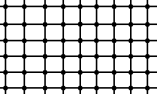
\includegraphics[width=7pc]{sqlattice.png}
	\end{minipage}\hspace{2pc}%
	\begin{minipage}{7pc}
		\caption{\label{label} 2d square lattice.}
	\end{minipage}\hspace{2pc}%
	\begin{minipage}{7pc}
		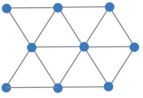
\includegraphics[width=7pc]{triangle-lattice.png}
	\end{minipage}\hspace{2pc}%
	\begin{minipage}{7pc}
		\caption{\label{label} 2d triangle lattice.}
	\end{minipage} 
\end{figure}

Hamiltonian of system is
%\begin{equation}
\[H = J\sum\limits_{ < i,j > } {({{\bf{\sigma }}_i}{{\bf{\sigma }}_j})} \label{ham}\]
%\end{equation}

where $<i,j>$ is spins of neighbor atoms. 
Scalar and mixed products of $\sigma$-matrices denoted as
\[\begin{array}{l}
({{\bf{\sigma }}_i}{{\bf{\sigma }}_j})\;\;\;\; = \;\;{\delta ^{\alpha \beta }} \cdot \sigma _i^\alpha  \otimes \sigma _j^\beta \\
({{\bf{\sigma }}_i}{{\bf{\sigma }}_j}{{\bf{\sigma }}_k}) = {\varepsilon ^{\alpha \beta \gamma }} \cdot \sigma _i^\alpha  \otimes \sigma _j^\beta  \otimes \sigma _k^\gamma \\
\alpha ,\beta ,\gamma  \in \{ x,y,z\} 
\end{array}
\label{products}
\]

A variational {\it upper} bound on the ground state energy $E_{\rm gs}$ of a quantum system, $E_{\rm gs} \leq \langle \Psi|H| \Psi \rangle$, is well-known.
Challenge of this paper is to find exact lower bound on the ground state energy per 1 site in thermodynamical limit
\[E_{\rm gs} \geqslant ?\]
In this paper we assume that $J=1$.

\section{Main ideas}
\subsection{Anderson bound \cite{Anderson}}
If we can divide full system to sum of subsystems, we can bound full ground state energy by ground state energies of subsystems:
\[{H_{full}} = \sum\limits_{i = 1}^M {{H_{i\;cl}}} \quad  \Rightarrow \quad {E_{gs\;full}}\;=\;\sum\limits_{i = 1}^M {{E_{i\;gs\;cl}}} \]
So we tessellate full lattice by small clusters, and we get full ground state energy per 1 site $E_{gs\;full}/N$ from 
ground state energies of clusters $E_{gs\;cl}$:
\[{E_{gs\;full}}/N\;=\frac{d}{m}{E_{gs\;cl}}\]
where
\begin{itemize}
	\item $N$ - number of spins in lattice
	\item $M$ - number of clusters
	\item $d$ - number of bonds per 1 site
	\item $m$ - number of bonds in cluster
\end{itemize}
\[M = \frac{{Nd}}{m} \label{MNdm} \]

\subsection{Variational method \cite{Baumgratz,Mazziotti}}
Ground state energy of full lattice can be expressed through a minimum over all density matrices ${\mathbb S}_{full}$, and it suffices to consider only those density matrices ${\mathbb S}_{full}^S$ that satisfy the same symmetries as the Hamiltonian:
\[E_{gs\;full} = \mathop {\min }\limits_\psi  \langle \psi |H|\psi \rangle  = 
\mathop{\min}\limits_{ \rho_{full} \in {\mathbb S}_{full}  } \mathop{\rm{tr}}_{full} H_{full} \rho _{full} = 
\mathop{\min}\limits_{ \rho_{full} \in {\mathbb S}_{full}^S} \mathop{\rm{tr}}_{full} H_{full} \rho _{full}
\]
The crystal lattice also is divided into identical clusters, which can be used to tile the entire lattice.
After that, under the trace, each expression ${H_{i\;cl}}{\rho _{full}}$ can be changed by a unitary transformation 
so that all ${H_{i\;cl}}$ match:
\[
 \mathop{\min}\limits_{ \rho _{full} \in {\mathbb S}_{full}^S} \mathop{\rm{tr}}_{full} H_{full} \rho_{full} = 
M\mathop{\min}\limits_{ \rho _{full} \in {\mathbb S}_{full}^S} \mathop{\rm{tr}}_{full} H_{cl}   \rho_{full}
\]
where $M$ - is number of clusters in lattice.
After that, the trace throughout the crystal can be divided into the sequential application of two partial traces on all the spins outside the cluster and only in the cluster:
\[
M\mathop{\min}\limits_{ \rho _{full} \in {\mathbb S}_{full}^S} \mathop{\rm{tr}}_{full} H_{cl} \rho _{full} = 
M\mathop{\min}\limits_{ \rho _{full} \in {\mathbb S}_{full}^S} \mathop{\rm{tr}}_{cl}
( H_{cl} \mathop{\rm{tr}}_{full\setminus cl} \rho _{full} )\]
Since the set of all cluster density matrices with symmetries of full lattice contains 
${\mathbb S}_{cl}^S \supset {\mathbb S}_{cl}^{tr\;S} = \{ 
{\mathop{\rm{tr}}_{ full \setminus cl}} \rho _{full} : \rho_{full} \in {\mathbb S}_{full}^S
\} $, so inequality arises for estimating the energy of the ground state of the crystal from below
\[E_{gs\;full} = 
M\mathop{\min}\limits_{ \rho _{cl} \in {\mathbb S}_{cl}^{tr\;S}} \mathop{\rm{tr}}_{cl} H_{cl} \rho _{cl} \geqslant
M\mathop{\min}\limits_{ \rho _{cl} \in {\mathbb S}_{cl}^S      } \mathop{\rm{tr}}_{cl} H_{cl} \rho _{cl} \]
or in another form
\[E_{gs\;full}/N\geqslant \frac{d}{m}
 \mathop{\min}\limits_{ \rho _{cl} \in {\mathbb S}_{cl}^S      } \mathop{\rm{tr}}_{cl} H_{cl} \rho _{cl} \]
where we use the same notations as in \eqref{MNdm}.

\subsection{Comparison}
Variational method in general outperform Anderson bound for the same cluster:
\[E_{gs\;cl} = 
 \mathop{\min}\limits_{ \rho _{cl} \in {\mathbb S}_{cl}  } \mathop{\rm{tr}}_{cl} H_{cl} \rho _{cl} \leqslant
 \mathop{\min}\limits_{ \rho _{cl} \in {\mathbb S}_{cl}^S} \mathop{\rm{tr}}_{cl} H_{cl} \rho _{cl} \]
where ${\mathbb S}_{cl}$ is set of all density matrices of cluster.

\section{Density matrix parametrization\cite{SqParam}}
Any density matrix must satisfy 3 conditions:
\[{\rho ^ + } = \rho ;\qquad \mathop{\rm{tr}}\rho  = 1;\qquad  \rho  \geqslant 0\]
If we take arbitrary hermitian matrix $\tau$, and square it and normalize it, we get valid density matrix:
\[\rho  = \frac{{{\tau ^2}}}{{\mathop{\rm{tr}}{\tau ^2}}};\qquad {\tau ^ + } = \tau \]

If Hamiltonian is invariant with respect of some symmetry group, then $\tau$ is also invariant with respect to the same symmetry group.

In our case, the Hamiltonian is spherically symmetric; therefore, the density matrix and $\tau$ can be expressed in terms of scalar and mixed products \eqref{products}.
Also our Hamiltonian is invariant with respect to time inverse, but mixed products are not; therefore, density matrix and $\tau$ can be expressed in terms of scalar products:
\[\begin{array}{l}
\rho  = \frac{1}{2^n} a_i A_i;\qquad \qquad \tau  = b_i A_i
\\
\{ A_i \}  = \{ 1,  \;\;({\bf \sigma}_j{\bf\sigma}_k), \;\;
({\bf \sigma}_j{\bf\sigma}_k)({\bf \sigma}_l{\bf\sigma}_m)\;\;,\;\;...\} 
\end{array}\]

Parameters $\tau$ $b_i$ run through all possible real values $a_i \in {\mathbb R}$.

Parameters $\rho$ $a_i$ is functions of $b_i$, and run through some subset ${a_i} = {f_i}(\{ b\} ) \in {\bf{V}} \subset {\mathbb R}$.
It is convex:
\[\forall {\rho _1},{\rho _2} \in V,\;\forall {a_1},{a_2} \ge 0\quad {a_1} + {a_2} = 1\;\; \Rightarrow \;\;{a_1}{\rho _1} + {a_2}{\rho _2} \in V\]
Its boundary is given by the formula
\[\partial {\bf{V}}:\;\det ||\frac{{\partial {a_i}}}{{\partial {b_j}}}|| = 0\]

\subsection{Symbolic relations and simplifications}
In Wolfram Mathematica was implemented (https://github.com/FeelUsM/ScalarMixedSpins) next operations:

Multiplication of scalar and mixed products, based on Pauli identity (${\sigma ^\alpha }{\sigma ^\beta } = {\delta ^{\alpha \beta }} + i{\varepsilon ^{\alpha \beta \gamma }}{\sigma ^\gamma }$), can be reduced to next formulas:
\[\begin{array}{l}
{({{\bf{\sigma }}_1}{{\bf{\sigma }}_2})^2}\qquad \quad {\mkern 1mu} {\mkern 1mu}  = \;\;{\mkern 1mu} 3 - 2({{\bf{\sigma }}_1}{{\bf{\sigma }}_2})\\
({{\bf{\sigma }}_1}{{\bf{\sigma }}_2})({{\bf{\sigma }}_2}{{\bf{\sigma }}_3})\;\;\;\; = \;\;\;({{\bf{\sigma }}_1}{{\bf{\sigma }}_3}) - i({{\bf{\sigma }}_1}{{\bf{\sigma }}_2}{{\bf{\sigma }}_3})\\
({{\bf{\sigma }}_1}{{\bf{\sigma }}_2})({{\bf{\sigma }}_1}{{\bf{\sigma }}_2}{{\bf{\sigma }}_3}) =  - ({{\bf{\sigma }}_1}{{\bf{\sigma }}_2}{{\bf{\sigma }}_3}) - 2i({{\bf{\sigma }}_1}{{\bf{\sigma }}_3}) + 2i({{\bf{\sigma }}_2}{{\bf{\sigma }}_3})\\
({{\bf{\sigma }}_1}{{\bf{\sigma }}_2}{{\bf{\sigma }}_3})({{\bf{\sigma }}_1}{{\bf{\sigma }}_2}) =  - ({{\bf{\sigma }}_1}{{\bf{\sigma }}_2}{{\bf{\sigma }}_3}) + 2i({{\bf{\sigma }}_1}{{\bf{\sigma }}_3}) - 2i({{\bf{\sigma }}_2}{{\bf{\sigma }}_3})\\
({{\bf{\sigma }}_1}{{\bf{\sigma }}_2})({{\bf{\sigma }}_2}{{\bf{\sigma }}_3}{{\bf{\sigma }}_4}) = ({{\bf{\sigma }}_1}{{\bf{\sigma }}_3}{{\bf{\sigma }}_4}) - i({{\bf{\sigma }}_1}{{\bf{\sigma }}_3})({{\bf{\sigma }}_2}{{\bf{\sigma }}_4}) + i({{\bf{\sigma }}_1}{{\bf{\sigma }}_4})({{\bf{\sigma }}_2}{{\bf{\sigma }}_3})\\
({{\bf{\sigma }}_2}{{\bf{\sigma }}_3}{{\bf{\sigma }}_4})({{\bf{\sigma }}_1}{{\bf{\sigma }}_2}) = ({{\bf{\sigma }}_1}{{\bf{\sigma }}_3}{{\bf{\sigma }}_4}) + i({{\bf{\sigma }}_1}{{\bf{\sigma }}_3})({{\bf{\sigma }}_2}{{\bf{\sigma }}_4}) - i({{\bf{\sigma }}_1}{{\bf{\sigma }}_4})({{\bf{\sigma }}_2}{{\bf{\sigma }}_3})\\
{({{\bf{\sigma }}_1}{{\bf{\sigma }}_2}{{\bf{\sigma }}_3})^2}{\mkern 1mu} {\mkern 1mu} {\mkern 1mu} \qquad {\mkern 1mu}  = 6 - 2({{\bf{\sigma }}_1}{{\bf{\sigma }}_2}) - 2({{\bf{\sigma }}_1}{{\bf{\sigma }}_3}) - 2({{\bf{\sigma }}_2}{{\bf{\sigma }}_3})\\
({{\bf{\sigma }}_1}{{\bf{\sigma }}_2}{{\bf{\sigma }}_3})({{\bf{\sigma }}_1}{{\bf{\sigma }}_2}{{\bf{\sigma }}_4}) =  - ({{\bf{\sigma }}_1}{{\bf{\sigma }}_3})({{\bf{\sigma }}_2}{{\bf{\sigma }}_4}) - ({{\bf{\sigma }}_1}{{\bf{\sigma }}_4})({{\bf{\sigma }}_2}{{\bf{\sigma }}_3}) + 2({{\bf{\sigma }}_3}{{\bf{\sigma }}_4}) + i({{\bf{\sigma }}_1}{{\bf{\sigma }}_3}{{\bf{\sigma }}_4}) + i({{\bf{\sigma }}_2}{{\bf{\sigma }}_3}{{\bf{\sigma }}_4})\\
({{\bf{\sigma }}_1}{{\bf{\sigma }}_2}{{\bf{\sigma }}_3})({{\bf{\sigma }}_1}{{\bf{\sigma }}_4}{{\bf{\sigma }}_5}) =  + ({{\bf{\sigma }}_2}{{\bf{\sigma }}_4})({{\bf{\sigma }}_3}{{\bf{\sigma }}_5}) - ({{\bf{\sigma }}_2}{{\bf{\sigma }}_5})({{\bf{\sigma }}_3}{{\bf{\sigma }}_4}) - i({{\bf{\sigma }}_1}{{\bf{\sigma }}_2})({{\bf{\sigma }}_3}{{\bf{\sigma }}_4}{{\bf{\sigma }}_5}) + i({{\bf{\sigma }}_1}{{\bf{\sigma }}_3})({{\bf{\sigma }}_2}{{\bf{\sigma }}_4}{{\bf{\sigma }}_5})
\end{array}\]
So if we have more than one same spin in term, we can reduce it.

In addition, in any term, we can leave only 1 mixed product:
\[{\rm{(}}{{\bf{\sigma }}_1}{{\bf{\sigma }}_2}{{\bf{\sigma }}_3}{\rm{)(}}{{\bf{\sigma }}_4}{{\bf{\sigma }}_5}{{\bf{\sigma }}_6}{\rm{) = }}\det \left( {\begin{array}{*{20}{c}}
	{{\rm{(}}{{\bf{\sigma }}_1}{{\bf{\sigma }}_4}{\rm{)}}}&{{\rm{(}}{{\bf{\sigma }}_2}{{\bf{\sigma }}_4}{\rm{)}}}&{{\rm{(}}{{\bf{\sigma }}_3}{{\bf{\sigma }}_4}{\rm{)}}}\\
	{{\rm{(}}{{\bf{\sigma }}_1}{{\bf{\sigma }}_5}{\rm{)}}}&{{\rm{(}}{{\bf{\sigma }}_2}{{\bf{\sigma }}_5}{\rm{)}}}&{{\rm{(}}{{\bf{\sigma }}_3}{{\bf{\sigma }}_5}{\rm{)}}}\\
	{{\rm{(}}{{\bf{\sigma }}_1}{{\bf{\sigma }}_6}{\rm{)}}}&{{\rm{(}}{{\bf{\sigma }}_2}{{\bf{\sigma }}_6}{\rm{)}}}&{{\rm{(}}{{\bf{\sigma }}_3}{{\bf{\sigma }}_6}{\rm{)}}}
	\end{array}} \right)
\label{mixeddet}
\]

We can introduce scalar product of matrices:
\[(A,B) \equiv \mathop{\rm{tr}}(A^+ B) = \mathop{\rm{tr}}(AB);\qquad {A^ + } = A\]
If sets of spins in $A$ and $B$ differ, then $(A,B) = 0$.
If $A$ and $B$ contains the same sets of spins, then $\left( {A,B} \right) = {2^N}{3^C}$,
where $N$ - is number of spins and $C$ - is the number of cycles arising from the imposition of bonds formed by scalar products:
\[{\rm{tr}}(\;({{\bf{\sigma }}_i}{{\bf{\sigma }}_j})({{\bf{\sigma }}_j}{{\bf{\sigma }}_k})...({{\bf{\sigma }}_l}{{\bf{\sigma }}_m})({{\bf{\sigma }}_m}{{\bf{\sigma }}_i})\;) = 3 \cdot {2^N}\]
-- for one cycle.
\[
{\rm{tr}}(\;({{\bf{\sigma }}_i}{{\bf{\sigma }}_j}{{\bf{\sigma }}_k})({{\bf{\sigma }}_i}{{\bf{\sigma }}_j}{{\bf{\sigma }}_n})\;({{\bf{\sigma }}_k}{{\bf{\sigma }}_l})...({{\bf{\sigma }}_m}{{\bf{\sigma }}_n})\;) = 
{\rm{tr}}(\;({{\bf{\sigma }}_i}{{\bf{\sigma }}_j}{{\bf{\sigma }}_k})({{\bf{\sigma }}_i}{{\bf{\sigma }}_j}{{\bf{\sigma }}_k})\;) = 6 \cdot {2^N}
\]

\subsection{Properties of basis}
Let us append into basis $\{A_i\}$ next elements:
$$
\{ B_i \}  = \{ ({\bf \sigma}_p{\bf\sigma}_r{\bf\sigma}_s),\;\;
({\bf \sigma}_p{\bf\sigma}_r{\bf\sigma}_s)({\bf \sigma}_j{\bf\sigma}_k), \;\;
({\bf \sigma}_p{\bf\sigma}_r{\bf\sigma}_s)({\bf \sigma}_j{\bf\sigma}_k)({\bf \sigma}_l{\bf\sigma}_m)\;\;,\;\;...\} 
$$

Basis $\{A_i\}$ or $\{A_i,B_j\}$ is not orthogonal, for example
\[\begin{array}{l}
\qquad \qquad \quad {\rm{A = (}}{{\bf{\sigma }}_1}{{\bf{\sigma }}_2}{\rm{)(}}{{\bf{\sigma }}_3}{{\bf{\sigma }}_4}{\rm{)}}\\
\qquad \qquad \quad {\rm{B = (}}{{\bf{\sigma }}_1}{{\bf{\sigma }}_3}{\rm{)(}}{{\bf{\sigma }}_2}{{\bf{\sigma }}_4}{\rm{)}}\\
\qquad \qquad \quad {\rm{C = (}}{{\bf{\sigma }}_1}{{\bf{\sigma }}_4}{\rm{)(}}{{\bf{\sigma }}_2}{{\bf{\sigma }}_3}{\rm{)}}\\
g = \left( {\begin{array}{*{20}{c}}
	{(AA)}&{(AB)}&{(AC)}\\
	{(BA)}&{(BB)}&{(BC)}\\
	{(CA)}&{(CB)}&{(CC)}
	\end{array}} \right) = \left( {\begin{array}{*{20}{c}}
	9&3&3\\
	3&9&3\\
	3&3&9
	\end{array}} \right) > 0
\end{array}\]

Also it is over-complete; however, all linear dependencies within the basis can be described by one formula:
\[{\rm{ + (}}{{\bf{\sigma }}_1}{{\bf{\sigma }}_2}{\rm{)(}}{{\bf{\sigma }}_3}{{\bf{\sigma }}_4}{{\bf{\sigma }}_5}{\rm{) - (}}{{\bf{\sigma }}_1}{{\bf{\sigma }}_3}{\rm{)(}}{{\bf{\sigma }}_2}{{\bf{\sigma }}_4}{{\bf{\sigma }}_5}{\rm{)}} + {\rm{(}}{{\bf{\sigma }}_1}{{\bf{\sigma }}_4}{\rm{)(}}{{\bf{\sigma }}_2}{{\bf{\sigma }}_3}{{\bf{\sigma }}_5}{\rm{) - (}}{{\bf{\sigma }}_1}{{\bf{\sigma }}_5}{\rm{)(}}{{\bf{\sigma }}_2}{{\bf{\sigma }}_3}{{\bf{\sigma }}_4}{\rm{)}} = 0
\label{basisdep}
\]
-- for elements with odd number of spins, and by the formula:
\[\det \left( {\begin{array}{*{20}{c}}
	{{\rm{(}}{{\bf{\sigma }}_1}{{\bf{\sigma }}_5}{\rm{)}}}&{{\rm{(}}{{\bf{\sigma }}_2}{{\bf{\sigma }}_5}{\rm{)}}}&{{\rm{(}}{{\bf{\sigma }}_3}{{\bf{\sigma }}_5}{\rm{)}}}&{{\rm{(}}{{\bf{\sigma }}_4}{{\bf{\sigma }}_5}{\rm{)}}}\\
	{{\rm{(}}{{\bf{\sigma }}_1}{{\bf{\sigma }}_6}{\rm{)}}}&{{\rm{(}}{{\bf{\sigma }}_2}{{\bf{\sigma }}_6}{\rm{)}}}&{{\rm{(}}{{\bf{\sigma }}_3}{{\bf{\sigma }}_6}{\rm{)}}}&{{\rm{(}}{{\bf{\sigma }}_4}{{\bf{\sigma }}_6}{\rm{)}}}\\
	{{\rm{(}}{{\bf{\sigma }}_1}{{\bf{\sigma }}_7}{\rm{)}}}&{{\rm{(}}{{\bf{\sigma }}_2}{{\bf{\sigma }}_7}{\rm{)}}}&{{\rm{(}}{{\bf{\sigma }}_3}{{\bf{\sigma }}_7}{\rm{)}}}&{{\rm{(}}{{\bf{\sigma }}_4}{{\bf{\sigma }}_7}{\rm{)}}}\\
	{{\rm{(}}{{\bf{\sigma }}_1}{{\bf{\sigma }}_8}{\rm{)}}}&{{\rm{(}}{{\bf{\sigma }}_2}{{\bf{\sigma }}_8}{\rm{)}}}&{{\rm{(}}{{\bf{\sigma }}_3}{{\bf{\sigma }}_8}{\rm{)}}}&{{\rm{(}}{{\bf{\sigma }}_4}{{\bf{\sigma }}_8}{\rm{)}}}
	\end{array}} \right) = 0\]
-- for elements with even number of spins, but the last formula is a consequence \eqref{mixeddet} and \eqref{basisdep}.
This statement was tested up to 10 spins. Its extrapolation to a greater number of spins is a mathematical hypothesis.
By compiling a Gram matrix, one can always get rid of overflow vectors. In the future we will assume that we have prepared an uncrowded basis.

The number of elements in the basis $\{A_i\}$ without taking into account over-complete is equal to
\[K(N)=C_N^{2k}(2k-1)!!\]
where $C_N^{2k}$ - binomial coefficient, $N$ is number of spins and $k$ is number of considered pairs.
$K(N)$ grows faster then exponentially (see table \ref{KN}).

\begin{table}
	\caption{\label{KN}Dependencies size of basis from number of spins.}
	\begin{center}
		\begin{tabular}{lllllllllllllllllllllllllllllll}
			\br
			$N$&2 &3 &4 &5 &10 &15 &20 &30 &40 &50 &60 \\
			\mr
			$K(N)$&1 &3 &9 &25 &9495 &1E+7 &2E+10 &6E+17 &7E+25 &2E+34 &2E+43 \\
			$4^N$&16&64&256&1024&1048576&1E+9&1E+12&1E+18&1E+24&1E+30&1E+36\\
			\br
		\end{tabular}
	\end{center}
\end{table}

\section{Examples and results}
Let us consider 1d lattice and cluster with 4 spins.
\[{H_{cl}} = ({{\bf{\sigma }}_1}{{\bf{\sigma }}_2}) + ({{\bf{\sigma }}_2}{{\bf{\sigma }}_3}) + ({{\bf{\sigma }}_3}{{\bf{\sigma }}_4})\]
Basis will be
\[\begin{array}{l}
\{ {A_k}\}  = \{ 1,\;({{\bf{\sigma }}_1}{{\bf{\sigma }}_2}),\;({{\bf{\sigma }}_1}{{\bf{\sigma }}_3}),\;({{\bf{\sigma }}_1}{{\bf{\sigma }}_4}),\;({{\bf{\sigma }}_2}{{\bf{\sigma }}_3}),\;({{\bf{\sigma }}_2}{{\bf{\sigma }}_4}),\;({{\bf{\sigma }}_3}{{\bf{\sigma }}_4}),\;\\
\;\;\;\;\;\;\;\;\;\;\;\;\;\;\;({{\bf{\sigma }}_1}{{\bf{\sigma }}_2})({{\bf{\sigma }}_3}{{\bf{\sigma }}_4}),\;({{\bf{\sigma }}_1}{{\bf{\sigma }}_3})({{\bf{\sigma }}_2}{{\bf{\sigma }}_4}),\;({{\bf{\sigma }}_1}{{\bf{\sigma }}_4})({{\bf{\sigma }}_2}{{\bf{\sigma }}_3})\} 
\end{array}\]
Let apply squaring parametrization:
\[\tau  = {b_i}{A_i},\;\;\rho  = \frac{1}{{{2^4}}}{a_i}{A_i},\;\;\;\rho  = {\tau ^2}\;\; \Rightarrow \;\;{a_k} = {a_{k,ij}}{b_i}{b_j}\]
with normalization:
\[{a_1} = 1\]
Lattice symmetries:
\[{a_{(1,2)}} = {a_{(2,3)}} = {a_{(3,4)}};\;\;{a_{(1,3)}} = {a_{(2,4)}}\]
But Hamiltonian already has symmetries, which we can apply firstly:
\[1\leftrightarrow 4, \;2\leftrightarrow 2, \;\Rightarrow 
{b_{(1,2)}} = {b_{(3,4)}};\;\;{b_{(1,3)}} = {b_{(2,4)}}\;\Leftrightarrow\;
{a_{(1,2)}} = {a_{(3,4)}};\;\;{a_{(1,3)}} = {a_{(2,4)}}
\]
Next restriction remains:
\[a_{(1,2)}=a_{(2,3)}\]

We can use numerical methods for calculating 
\[\mathop {\min } \rm{tr}\;H\rho  = \mathop {\min }\limits_b \frac{{\eta _{ij}}{b_i}{b_j}}{{{\rm{a}}_{1,ij}}{b_i}{b_j}}\]
where ${\eta _{ij}} = Tr({A_i}H{A_j})$
with constraint
\[({a_{(1,2),ij}} - {a_{(2,3),ij}}){b_i}{b_j}=0\]

Results for clusters with 4,5,6 spins you can see in table \ref{result}.


\begin{table}
	\caption{\label{result}Results.}
	\begin{center}
		\begin{tabular}{lllllllllllllllllllllllllllllll}
			\br
			$N$&Anderson bound&variational method\\
			\mr
			4 &-2.1547  & -2.0\\
			5 &-1.92789 & -1.86852\\
			6 &-1.99486 & -1.86852\\
			\br
		\end{tabular}
	\end{center}
\end{table}

\section*{References}

\begin{thebibliography}{9}
\bibitem{SqParam} Il'in N, Shpagina E, Uskov F and Lychkovskiy O 2018
Squaring parametrization of constrained and unconstrained sets of quantum states
{\it J. Phys.} A: Math. Theor. {\bf 51}.085301

\bibitem{TarrachWalenti}
Tarrach R and Valent{\'\i} R 1990 
Exact lower bounds to the ground-state energy of spin systems: The two-dimensional S= 1/2 antiferromagnetic Heisenberg model
{\it Phys. Rev.} B {\bf 41(13)} 9611

\bibitem{Anderson} Anderson PW 1951
Limits on the energy of the antiferromagnetic Ground State
{\it Phys. Rev.} {\bf 83(6)} 1260

\bibitem{Baumgratz} Baumgratz T and Plenio MB 2012
Lower bounds for ground states of condensed matter systems
{\it New Journal of Physics} {\bf 14(2)} 023027

\bibitem{Mazziotti} Mazziotti DA 2002
Variational minimization of atomic and molecular ground-state energies via the two-particle reduced density matrix
{\it Phys.Rev.} A {\bf 65(6)} 062511

\bibitem{BeachSandvik} Beach KSD and Sandvik AW 2006
Some formal results for the valence bond basis
{\it Nuclear Physics} B {\bf 750(3)} 142–178

\bibitem{MattisPan} Mattis DC and Pan CY 1988
Ground-State Energy of Heisenberg antiferromagnet for Spins s=1/2 and s=1 in d=1 and 2 Dimensions
{\it Phys.Rev.Lett.} {\bf 61(4)} 463

%\bibitem{iopartnum} IOP Publishing is to grateful Mark A Caprio, Center for Theoretical Physics, Yale University, for %permission to include the {\tt iopart-num} \BibTeX package (version 2.0, December 21, 2006) with  this documentation. %Updates and new releases of {\tt iopart-num} can be found on \verb"www.ctan.org" (CTAN). 
\end{thebibliography}

%\printbibliography

\end{document}


